\subsection*{Task 4.2}

\subsubsection*{Task 4.2.1}
\begin{figure}[h]
	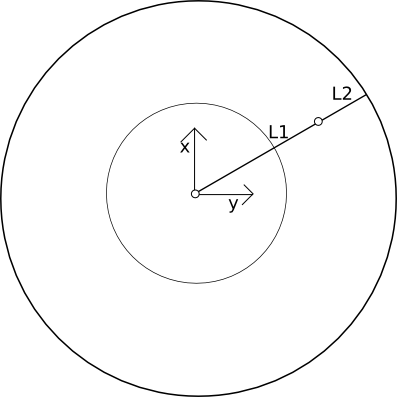
\includegraphics[scale=0.7]{4_2_1.png}
	\caption{The workspace of the 2-DOF planar robot}
	\label{fig:2dof-planar}
\end{figure}
The workspace is described by a circle. The distance of the inner and outer boundary of the workspace is then $2 \cdot l_2$.

\subsubsection*{Task 4.2.2}
The manipulator is similar to the one in Task 4.1, but has only 2 Joints. The resulting matrices $^0T_1$ and $^0T_2$ are the same.

\begin{align*}
^0T_1 &= 
\begin{pmatrix}
C1 & -S1 & 0 & l_1 C1\\
S1 &  C1 & 0 & l_1 S1\\
0  &  0  & 1 & 0\\
0  &  0  & 0 & 1
\end{pmatrix},
\,^0T_2 &= 
\begin{pmatrix}
C1C2-S1S2 & -C1S2-S1C2 & 0 & C1l_2C2-S1l_2S2+l_1C1\\
S1C2+C1S2 & -S1S2+C1C2 & 0 & S1l_2C2+C1l_2S2+l_1S1\\
0  &  0  & 1 & 0\\
0  &  0  & 0 & 1
\end{pmatrix}
\end{align*}

The $z_i$ and $o_i$ are then:

\begin{align*}
z_0 &= 
\begin{pmatrix}
0 \\ 0 \\ 1
\end{pmatrix},
z_1 = 
\begin{pmatrix}
0 \\ 0 \\ 1
\end{pmatrix}\\
o_1^0 &= 
\begin{pmatrix}
l_1C1 \\ l_1S1 \\ 0
\end{pmatrix},
o_2^0 = 
\begin{pmatrix}
C1l_2C2-S1l_2S2+l_1C1 \\ S1l_2C2+C1l_2S2+l_1S1 \\ 0
\end{pmatrix}\\
\end{align*}

\begin{align*}
J_{v_1} &= 
z_0\times (o_2^0-o_0^0)\\
 &=
\begin{pmatrix}
0 \\ 0 \\ 1
\end{pmatrix}\times\left(
\begin{pmatrix}
C1l_2C2-S1l_2S2+l_1C1 \\ S1l_2C2+C1l_2S2+l_1S1 \\ 0
\end{pmatrix}-
\begin{pmatrix}
0 \\ 0 \\ 0
\end{pmatrix}
\right) \\
 &= \begin{pmatrix}
 -S1l_2C2+C1l_2S2+l_1S1 \\ C1l_2C2-S1l_2S2-S1l_2S2-l_1C1 \\ 0
 \end{pmatrix} \\
 J_{v_2} &= 
z_1\times (o_2^0-o_1^0)\\
 &=
\begin{pmatrix}
0 \\ 0 \\ 1
\end{pmatrix}\times\left(
\begin{pmatrix}
C1l_2C2-S1l_2S2+l_1C1 \\ S1l_2C2+C1l_2S2+l_1S1 \\ 0
\end{pmatrix}-
\begin{pmatrix}
l_1C1 \\ l_1S1 \\ 0
\end{pmatrix}
\right) \\
 &= \begin{pmatrix}
0 \\ 0 \\ 1
\end{pmatrix}\times
\begin{pmatrix}
 C1l_2C2-S1l_2S2 \\ S1l_2C2+C1l_2S2 \\ 0
 \end{pmatrix} \\
 &= \begin{pmatrix}
 -S1l_2C2+C1l_2S2 \\ C1l_2C2 \\ 0
 \end{pmatrix} \\
 J_{w_1} &= J_{w_2} =  
\begin{pmatrix}
0 \\ 0 \\ 1
\end{pmatrix}
\end{align*}

The Jacobian is then:


\begin{flalign*}
J &=
\begin{pmatrix}
-S1l_2C2+C1l_2S2+l_1S1 & -S1l_2C2+C1l_2S2  \\
C1l_2C2-S1l_2S2-S1l_2S2-l_1C1 & C1l_2C2  \\
0 & 0  \\
0 & 0  \\
0 & 0  \\
1 & 1 
\end{pmatrix}	
\end{flalign*}

\subsubsection*{Task 4.2.3}
To determine the singular configurations we would need to calculate where the Jacobian is not invertible. For square matrices this is the case when the determinant is zero. We do not have a square matrix, so it is generally not invertible, but we can reduce it to the first two rows and columns to get a square matrix.
We have to calculate:\\
\begin{align*}
0 &= det \left( 
\begin{pmatrix}
-S1l_2C2+C1l_2S2+l_1S1 & -S1l_2C2+C1l_2S2 \\
C1l_2C2-S1l_2S2-S1l_2S2-l_1C1 & C1l_2C2
\end{pmatrix} 
\right) \\
 &=
 (-S1l_2C2+C1l_2S2+l_1S1)*C1l_2C2 - (-S1l_2C2+C1l_2S2)*(C1l_2C2-S1l_2S2-S1l_2S2-l_1C1)
\end{align*}

Which should resolve to $\theta_2$ being zero$\degree$ or 180$\degree$. \\

TODO: Further simplifications to make the conclusion more obvious???

\subsubsection*{Task 4.2.4}

Both singular configurations are workspace boundary singularities. The arm is either fully extended at $\theta_2 = 0\degree$ or fully folded onto itself at $\theta_2 = 180\degree$. The arm then describes the outer and inner circle of its workspace.